\documentclass[a4paper,twoside,12pt]{book}



\usepackage[printonlyused,footnote]{acronym}
\usepackage{amsmath}
\usepackage{amssymb}
\usepackage{amsthm}
\usepackage[title]{appendix}
\usepackage[style=iso-numeric, 
    backend=biber, 
    language=czech
    ]{biblatex}
\usepackage[font=small,
    labelfont=bf]{caption}
\usepackage{csquotes}
\usepackage[resetfonts]{cmap}
\usepackage{emptypage}
\usepackage{fancyhdr}
\usepackage{float}
\usepackage[T1]{fontenc}            % font encoding
\usepackage{gensymb}
\usepackage[a4paper,
    hmarginratio=3:2
]{geometry}                         % geometry of page, margins etc.
\usepackage{graphicx}
\usepackage[hidelinks,
    unicode]{hyperref}              % clickable links
\usepackage{import}
\usepackage{indentfirst}
\usepackage[utf8]{inputenc}         % UTF-8 character set
\usepackage{listings}
\usepackage{lmodern}
\usepackage{makecell}               % for tables
\usepackage[version=3]{mhchem}
\usepackage{paralist}
\usepackage{pdfpages}
\usepackage{tabularx} 
\usepackage[nottoc]{tocbibind}      % citations
\usepackage{tocloft}
\usepackage{upgreek}
\usepackage{xargs}
%%% Specification of all necessary stuff %%%
% ========================================


% Specification of the author and consultants
\newcommand{\autor}{Thesis Author}   % vyplňte své jméno a příjmení (s akademickým titulem, máte-li jej)
\newcommand{\woman}{} % pokud jste ŽENA, ZMĚŇTE na: ...{\woman}{a} (je to do Prohlášení)

\newcommand{\vedouci}{title. Great Supervisor} % vyplňte jméno a příjmení vedoucího práce, včetně titulů, např.: Doc. Ing. Ivo Malý, Ph.D.
\newcommand{\pracovisteVed}{Awesome and Rich company from Supervisor} % ZMĚŇTE, pokud vedoucí Vaší práce není z KSI
\newcommand{\konzultant}{title. Talkative Consultant} % POKUD MÁTE určeného konzultanta, NAPIŠTE jeho jméno a příjmení
\newcommand{\pracovisteKonz}{Very consultive Group} % POKUD MÁTE konzultanta, NAPIŠTE jeho pracoviště
\newcommand{\konzultantt}{title. Awesome SecondOne} % POKUD MÁTE určeného konzultanta, NAPIŠTE jeho jméno a příjmení
\newcommand{\pracovisteKonzt}{The second Group} % POKUD MÁTE konzultanta, NAPIŠTE jeho pracoviště

% Specification of thesis -- copy and paste from your task list
\newcommand{\nazevcz}{Název česky}
\newcommand{\nazeven}{Název anglicky}
\newcommand{\rok}{2020}  % rok odevzdání práce (jen rok odevzdání, nikoli celý akademický rok!)
\newcommand{\skola}{School name (see commands.tex for acronyms)}
\newcommand{\fakulta}{Faculty name (see commands.tex for acronyms)}
\newcommand{\katedra}{Department name (see commands.tex for acronyms)}
\newcommand{\kde}{Praze} % studenti z Děčína ZMĚNÍ na: "Děčíně" (doplní se k "prohlášení")
\newcommand{\program}{Aplikace přírodních věd} % změňte, pokud máte jiný stud. program
\newcommand{\obor}{Jaderné inženýrství} % změňte, pokud máte jiný obor

%% LANGUAGE SETTINGS
% Uncomment exactly one block

%==================
%% CZECH
\usepackage[czech]{babel} % česky psaná práce, typografická pravidla. Překládejte pomocí "latex.exe" nebo "pdflatex.exe"

% Uncomment exactly one 
\newcommand{\druh}{Bakalářská práce} 
%\newcommand{\druh}{Výzkumný úkol} 
%\newcommand{\druh}{Diplomová práce}
%==================

%==================
%% SLOVAK
% \usepackage[slovak]{babel} 
%==================


%==================
%% ENGLISH
% \usepackage[english]{babel}

% Uncomment exactly one 
%\newcommand{\druh}{Bachelor thesis} 
%\newcommand{\druh}{Research project} 
%\newcommand{\druh}{Master thesis}
%==================



% Insert scan of your task -- put it in "img" folder -- 2 separate PDFs recommended
\newcommand{\skenZadaniPredni}{specimen1.pdf}
\newcommand{\skenZadaniZadni}{specimen2.pdf}

% Keywords in zde NAPIŠTE česky max. 5 klíčových slov AND translate them into english
\newcommand{\klicova}{slovo1, slovo2, slovo3}  
\newcommand{\keyword}{keyword1, keyword2, keyword3}
\newcommand{\abstrCZ}{% zde NAPIŠTE abstrakt v češtině (cca 7 vět, min. 80 slov)
Tato práce se zabývá psaním závěrečných prací.
}
\newcommand{\abstrEN}{% zde NAPIŠTE abstrakt v angličtině
The thesis deals with the issue of thesis writing. 
}
\newcommand{\prohlaseni}{% text prohlášení můžete mírně upravit
Prohlašuji, že jsem svou bakalářskou práci vypracoval\woman{} samostatně a použil\woman{} jsem pouze podklady (literaturu, projekty, SW atd.) uvedené v přiloženém seznamu.
} 
\newcommand{\podekovani}{%Podekovani se doporucuje neprehanet
 Děkuji Ing. Eleonoře Krtečkové, Ph.D. za vedení mé bakalářské práce a za podnětné návrhy, které ji obohatily.
% NEBO:
% Děkuji vedoucímu práce doc. Pafnutijovi Snědldítětikaši, Ph.D. za neocenitelné rady a pomoc při tvorbě bakalářské práce.
}

% Page style -- uncomment exactly one
% 
% Style 1 -- fancy -- nice looking, but unfortunatelly, not debugged yet :(
% \pagestyle{fancy}
% \fancyfoot{}
% \fancyhead[RO,LE]{\thepage}
% \fancyhead[RE]{\nouppercase{\leftmark}}
% \fancyhead[LO]{\nouppercase{\rightmark}}

% Style 2 -- plain
\pagestyle{plain}      % stránky číslované dole uprostřed


% Page numbering
\pagenumbering{arabic} % číslování stránek arabskými číslicemi

% Depth of table of contents (ToC) (2 is RECOMMENDED, other are believed to be confusing and poorly arranged!
% 0 = only parts and chapters are included in ToC
% 1 = parts, chapters, sections
% 2 = parts, chapters, sections, subsections
% 3 = parts, chapters, sections, subsections, subsubsections
\setcounter{tocdepth}{2}


% Margins 
\topmargin=-10mm      % horní okraj trochu menší
\textwidth=150mm      % šířka textu na stránce
\textheight=250mm     % "výška" textu na stránce

% Intendation
\parindent=0pt % odsazení 1. řádku odstavce
\parskip=7pt   % mezera mezi odstavci

% Font size
\renewcommand\cftchapfont{\small\bfseries}
\renewcommand\cftsecfont{\footnotesize}
\renewcommand\cftsubsecfont{\footnotesize}

\renewcommand\cftchappagefont{\small\bfseries}
\renewcommand\cftsecpagefont{\footnotesize}
\renewcommand\cftsubsecpagefont{\footnotesize}

% Spacing
\frenchspacing % za větou bude mezislovní mezera (v anglických textech je mezera za větou delší)
\widowpenalty=1000 % "síla" zákazu vdov (= jeden řádek ze začátku odstavce na konci stránky)
\clubpenalty=1000 % "síla" zákazu sirotků (= jeden řádek/slovo z konce odstavce samostatně na začátku stránky)
\brokenpenalty=1000 % "síla" zákazu zlomu stránky za řádkem, který má na konci rozdělené slovo

% Aliases

%% Font
\newcommand{\bv}{\mathbf} % bold math
\newcommand{\tb}{\textbf} % bold font
\newcommand{\ti}{\textit} % itallic font

%% Paralist environments
%%% shorter compactenum
\newcommandx{\cen}[1]{
    \begin{compactenum}
        #1
    \end{compactenum}
}
%%% shorter compactitem
\newcommandx{\cit}[1]{
    \begin{compactitem}
        #1
    \end{compactitem}
}

% Commands

%% Graphics

%%% Single figure
    \newcommandx{\pic}[5][4=0.8,5=H]{%
        \begin{figure}[#5]
            \centering
            \includegraphics[width=#4\textwidth]{./img/#1}
            \caption[#2]{#3}
            \label{#1}
        \end{figure}
    }

    %%% Two pictures side-by-side
    \newcommandx{\dpic}[9][7=0.49,8=0.98,9=H]{%
        \begin{figure}[#9]
            \centering
            \begin{minipage}{#7\textwidth}
                \centering
                \includegraphics[width=#8\textwidth]{img/#1} % first figure itself
                \caption[#3]{#4}
                \label{#1}
            \end{minipage}\hfill
            \begin{minipage}{#7\textwidth}
                \centering
                \includegraphics[width=#8\textwidth]{img/#2} % second figure itself
                \caption[#5]{#6}
                \label{#2}
            \end{minipage}
        \end{figure}
    }

    %%% Three figures side-by-side... Not really sure, whether it looks good
    \newcommandx{\tpic}[9]{%
        \begin{figure}[H]
            \centering
            \begin{minipage}{0.3\textwidth}
                \centering
                \includegraphics[width=0.95\textwidth]{img/#1} % first figure itself
                \caption[#2]{#3}
                \label{#1}
            \end{minipage}\hfill
            \begin{minipage}{0.3\textwidth}
                \centering
                \includegraphics[width=0.95\textwidth]{img/#4} % second figure itself
                \caption[#5]{#6}
                \label{#4}
            \end{minipage}\hfill
            \begin{minipage}{0.3\textwidth}
                \centering
                \includegraphics[width=0.95\textwidth]{img/#7} % second figure itself
                \caption[#8]{#9}
                \label{#7}
            \end{minipage}
        \end{figure}
    }

%% Better footnotes above punctuation
\newcommand{\footnotei}[2]{%
    \mbox{%
        \setbox0\hbox{#1}%
        \copy0%
        \hspace{-\wd0}}%
    \footnote{#2}%
}

%% Equations
\newcommandx{\eq}[1]{
    \begin{equation}
        #1
    \end{equation}
}
\newcommandx{\eqa}[1]{
    \begin{align}
        #1
    \end{align}
}

%% Units
\newcommand{\jdt}[1]{
    $\mathrm{#1}$
}

\newcommand{\jde}[1]{
    \mathrm{#1}
}

%% Derivative faster
\newcommand{\der}[2]{
    \frac{\mathrm{d} #1}{\mathrm{d} #2}
}

%% N-th derivative faster
\newcommand{\nder}[3]{
    \frac{\mathrm{d}^{#3} #1}{\mathrm{d} {#2}^{#3}}
}

%% Partial derivative faster
\newcommand{\pder}[2]{
    \frac{\partial #1}{\partial #2}
}

%% N-th partial derivative faster
\newcommand{\npder}[3]{
    \frac{\partial^{#3} #1}{\partial {#2}^{#3}}
}

%% Auto-sized brackets
\renewcommand{\(}{
    \left(
}
\renewcommand{\)}{
    \right)
}

\renewcommand{\[}{
\left[
}
\renewcommand{\]}{
    \right]
}

% \_ for non-itallic sub indices
\let\underscore\_                                           % underscore sign
\let\xor\^                                                  % xor sign
\renewcommand\_[2][1]{\ifmmode _{\textnormal{\scalebox{#1}{#2}}}\else\underscore#2\fi} %roman subscript
\renewcommand\^[2][1]{\ifmmode ^{\textnormal{\scalebox{#1}{#2}}}\else\xor#2\fi} %roman superscript
\def\smallind{0.8}

%% Math aliases
\newcommand{\mdef}[3]{
	\begin{define}[#1]
		\label{mdef:#2}
		#3
	\end{define}
}

\newcommand{\mtheor}[3]{
	\begin{theorem}[#1]
		\label{mtheor:#2}
		#3
	\end{theorem}
}

\newcommand{\mlemma}[3]{
	\begin{lemma}[#1]
		\label{mlemma:#2}
		#3
	\end{lemma}
}

\newcommand{\mcomm}[3]{
	\begin{comment}[#1]
		\label{mcomm:#2}
		#3
	\end{comment}
}

\newcommand{\mex}[2]{
	\begin{example}
		\label{mex:#1}
		#2
	\end{example}
}


\begin{document}

\newcommand{\logoCVUT}{
\includegraphics{img/symbol_cvut_konturova_verze_cb.pdf}} % logo ČVUT -- podle grafického manuálu ČVUT platného od prosince 2016. Pokud nevyhovuje PDF-verze, tak použijte jinou variantu loga: https://www.cvut.cz/logo-a-graficky-manual -> "Symbol a logo ČVUT v Praze"). Pokud chcete logo úplně vynechat, zadejte místo "\includegraphics{...}" text "\vspace{35mm}"

\frontmatter

\thispagestyle{empty}

\begin{center}
	{\LARGE
		\cvut\par
		\fjfi
	}
    \vspace{10mm}

    \begin{tabular}{c}
		\tb{\kjr} \\[3pt]   
		\tb{Obor: \obor}\\
    \end{tabular}

   \vspace{10mm} \logoCVUT \vspace{15mm} 

   {\huge \tb{\nazevcz}\par}
   \vspace{5mm}   
   {\huge \tb{\nazeven}\par}
   
   \vspace{15mm}
   {\Large \MakeUppercase{\druh}}

   \vfill
   {\large
    \begin{tabular}{ll}
    Vypracoval: & \autor\\
    Vedoucí práce: & \vedouci\\
    Rok: & \rok
    \end{tabular}
   }
\end{center}

\clearpage{\pagestyle{empty}\cleardoublepage} % prázdná stránka za tou "titulní", bez čísla

%%%%%%%%%%%% ZADÁNÍ PRÁCE %%%%%%%%%%%%
% Zadání (podepsané děkanem!) musíte NASKENOVAT. Ideálně jako 2stránkové PDF (soubor "zadani_cele.pdf"). 
% Před svázáním to v jednom výtisku VYMĚNÍTE ZA ORIGINÁLNÍ ZADÁNÍ (podepsané děkanem fakulty)!
\newpage  % SEM NESAHEJTE!
\thispagestyle{empty} % SEM NESAHEJTE!

%% zde podle toho, jak jste zadání naskenovali, VYBERTE variantu A, B nebo C:
%
% --- varianta A: zadání naskenované jako 2stránkové PDF:
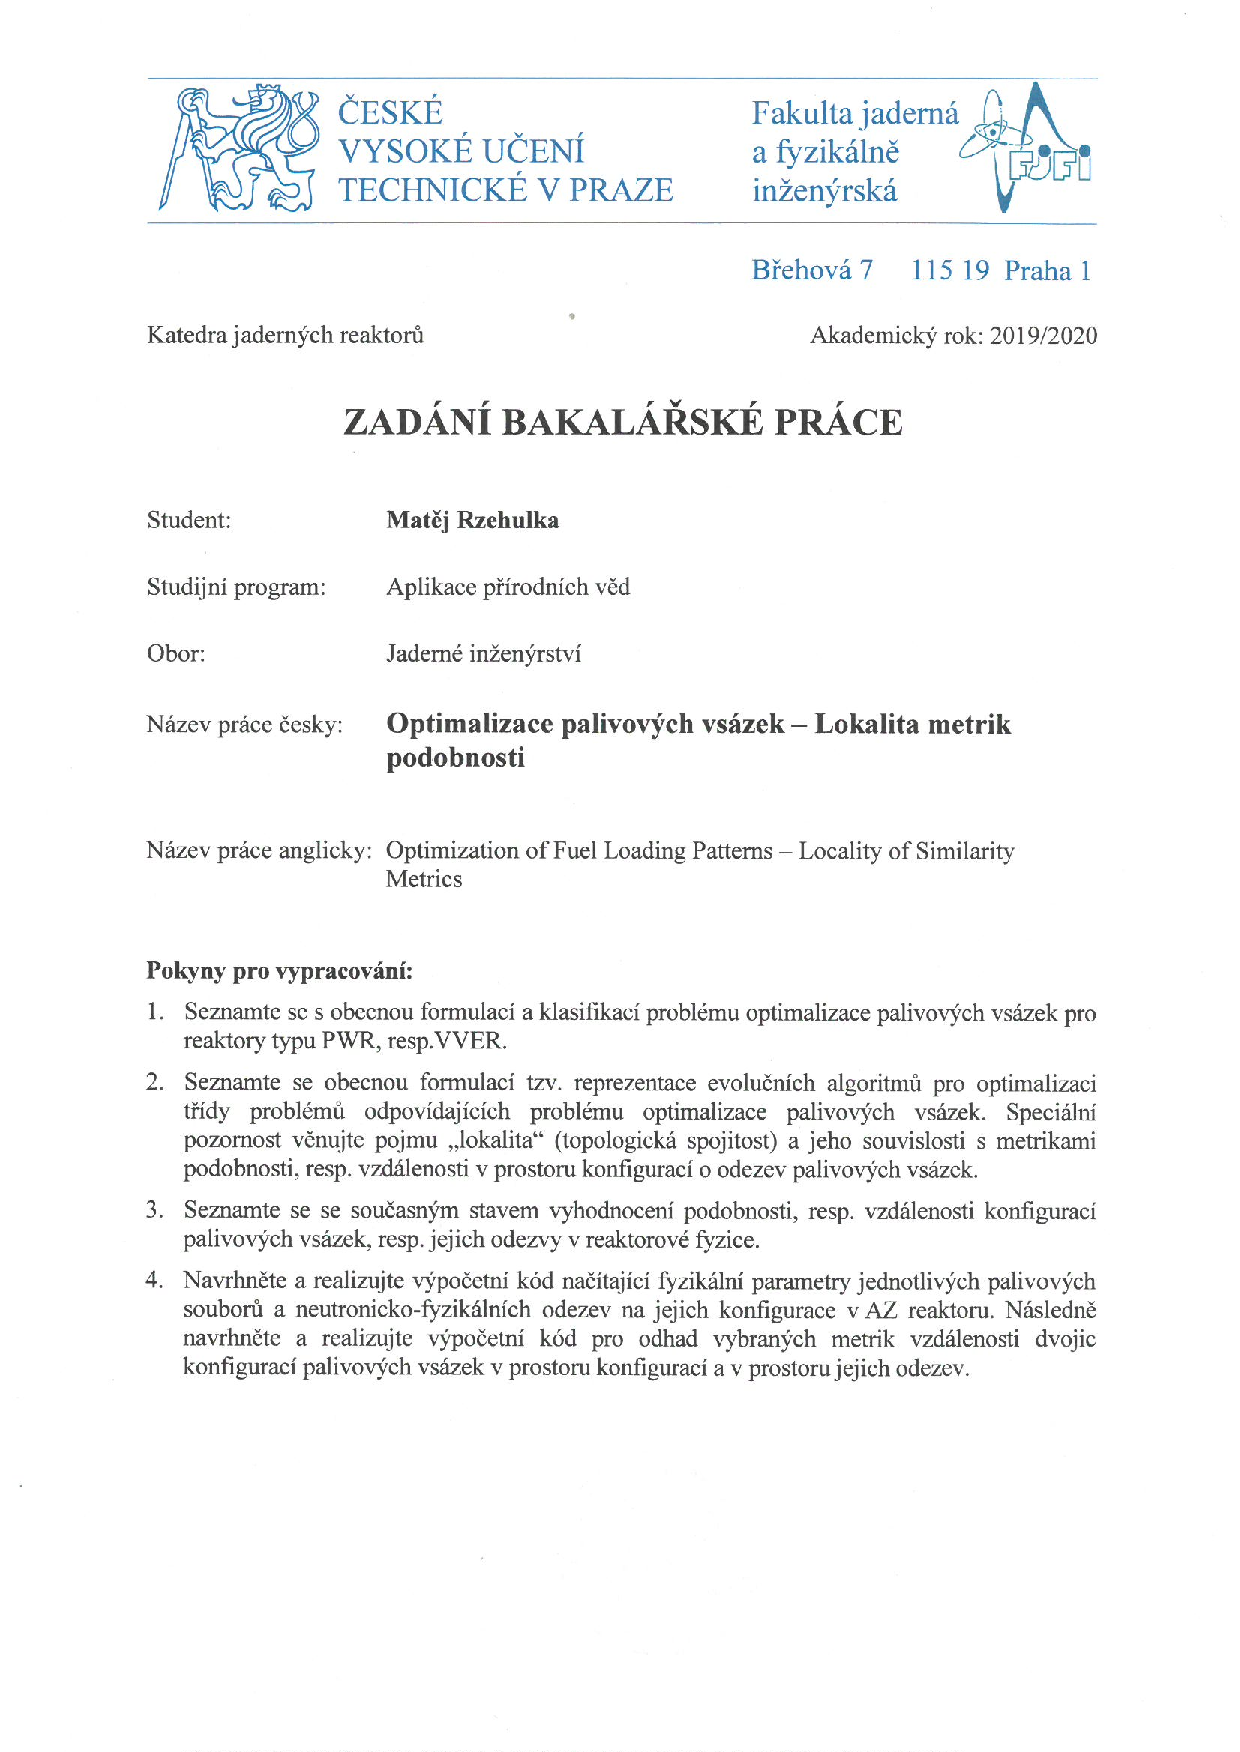
\includepdf[pages={1}]{img/bp-rzehulka-zad1.pdf} % NAHRAĎTE správným souborem!
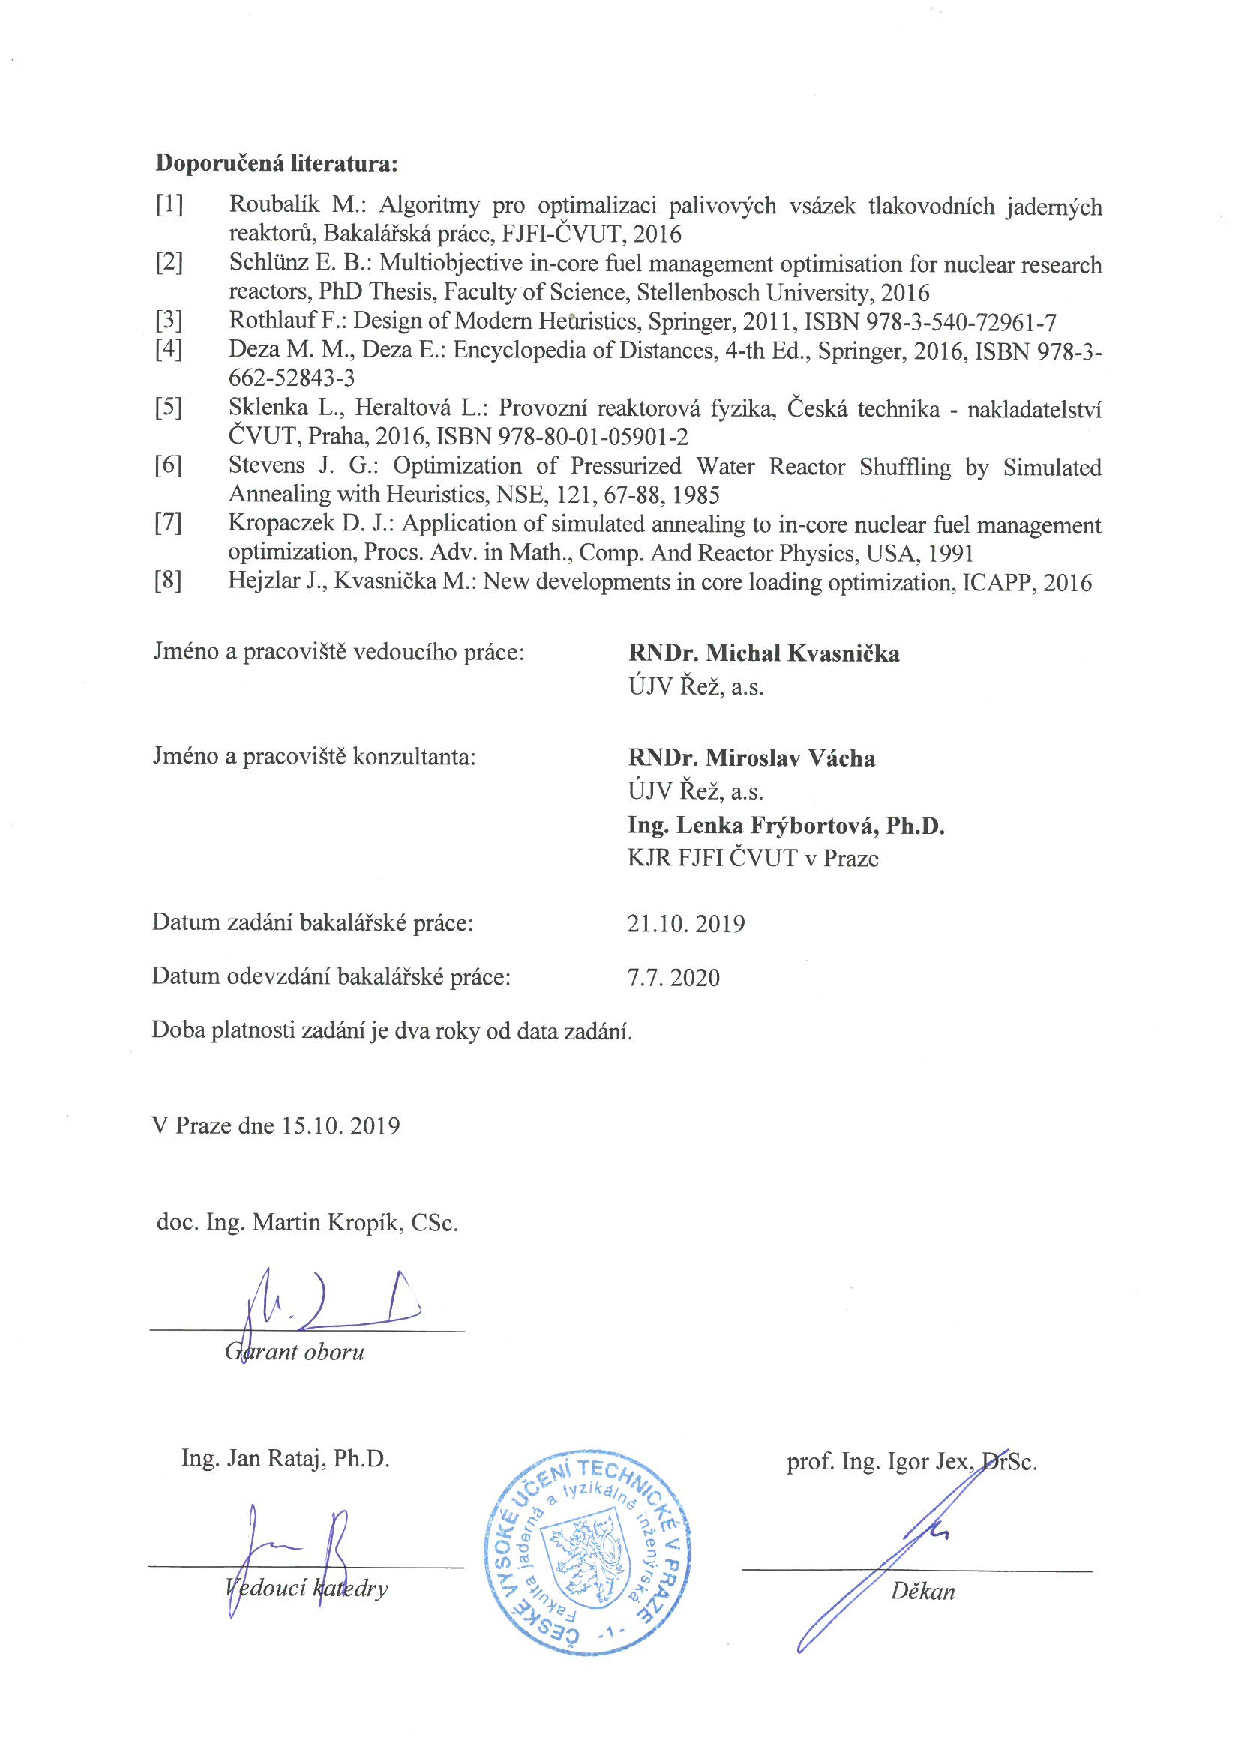
\includepdf[pages={1}]{img/bp-rzehulka-zad2.pdf}
%
%% --- varianta B: zadání naskenované jako jednotlivé stránky:
%\includepdf[pages={1}]{zadani1.pdf} % 1. strana zadání v PDF
%\includepdf[pages={1}]{zadani2.pdf} % 2. strana zadání v PDF
%
%% --- varianta C: zadání naskenované jako 2 samostatné obrázky:
%% 1. strana zadání
%\begin{center}
%     \includegraphics[width=1\textwidth]{zadani1.jpg}
%\end{center}
%% 2. strana zadání
%\newpage  % SEM NESAHEJTE!
%\thispagestyle{empty} % SEM NESAHEJTE!
%\begin{center}
%     \includegraphics[width=1\textwidth]{zadani2.jpg}
%\end{center}


%%%%%%%%%%%% Prohlášení -- SEM NESAHEJTE! Generuje se automaticky z výše nastavených maker \kde{} a \prohlaseni{}. %%%%%%%%%%%%
\newpage % SEM NESAHEJTE!
\thispagestyle{empty}  % SEM NESAHEJTE!

% SEM NESAHEJTE!
~
\vfill % prázdné místo. SEM NESAHEJTE!

\tb{Prohlášení} % SEM NESAHEJTE!

\vspace{1em} % vertikální mezera. SEM NESAHEJTE!
\prohlaseni

\vspace{2em}  % SEM NESAHEJTE!
\hspace{-0.5em}\begin{tabularx}{\textwidth}{X c}  % SEM NESAHEJTE!
V \kde\ dne .................... &........................................ \\	% SEM NESAHEJTE!
	& \autor
\end{tabularx}	% SEM NESAHEJTE!


%%%%%%%%%%%% Poděkování  %%%%%%%%%%%%
\newpage
\thispagestyle{empty}

~
\vfill % prázdné místo


% -- následující kus kódu (do "%%%%%%%%%%%% ABSTRAKT") můžete odstranit, pokud nechcete psát poděkování:
\tb{Poděkování}

\vspace{1em} % vertikální mezera
\podekovani
\begin{flushright}
\autor
\end{flushright}  % <------- tady končí stránka s poděkováním


%%%%%%%%%%%% ABSTRAKT atp. Je generován AUTOMATICKY podle maker nastavených na začátku souboru) %%%%%%%%%%%% 
\newpage   % SEM NESAHEJTE!
\thispagestyle{empty}   % SEM NESAHEJTE!

% příprava:    (na následujících 8 řádků NESAHEJTE!)
\newbox\odstavecbox
\newlength\vyskaodstavce
\newcommand\odstavec[2]{%
    \setbox\odstavecbox=\hbox{%
         \parbox[t]{#1}{#2\vrule width 0pt depth 4pt}}%
    \global\vyskaodstavce=\dp\odstavecbox
    \box\odstavecbox}
\newcommand{\delka}{120mm} % šířka textů ve 2. sloupci tabulky

% použití přípravy:    % dovnitř "tabular" vůbec NESAHEJTE!
\begin{tabular}{ll}
  {\em Název práce:} & ~ \\
  \multicolumn{2}{l}{\odstavec{\textwidth}{\textbf \nazevcz}} \\[1em]
  {\em Autor:} & \autor \\[1em]
  {\em Studijní program:} & \program \\
  {\em Obor:} & \obor \\
  {\em Druh práce:} & \druh \\[1em]
  {\em Vedoucí práce:} & \odstavec{\delka}{\vedouci\\ \pracovisteVed} \\
  {\em Konzultant:} & \odstavec{\delka}{\konzultant \\ \pracovisteKonz}  % VYMAŽTE text "-- %" v případě, že jste neměli konzultanta
 \\[1em]
  & \odstavec{\delka}{\konzultantt \\ \pracovisteKonzt} \\[1em]
  \multicolumn{2}{l}{\odstavec{\textwidth}{{\em Abstrakt:} ~ \abstrCZ  }} \\[1em]
  {\em Klíčová slova:} & \odstavec{\delka}{\klicova} \\[2em]

  {\em Title:} & ~\\
  \multicolumn{2}{l}{\odstavec{\textwidth}{\textbf \nazeven}}\\[1em]
  {\em Author:} & \autor \\[1em]
  \multicolumn{2}{l}{\odstavec{\textwidth}{{\em Abstract:} ~ \abstrEN  }} \\[1em]
  {\em Key words:} & \odstavec{\delka}{\keyword}
\end{tabular}



%%%%%%%%%%%% Obsah práce ... je generován AUTOMATICKY %%%%%%%%%%%%

\newpage  % SEM NESAHEJTE!
\parskip=0pt
\begin{small}
\tableofcontents % SEM NESAHEJTE!
\end{small}
\parskip=7pt
\newpage % SEM NESAHEJTE!


%--------------------------------------------------------
%|         Zde začíná SAMOTNÁ PRÁCE (text)              |
%--------------------------------------------------------

\chapter*{\AcronymsWord}
\addcontentsline{toc}{chapter}{\AcronymsWord}
\markboth{\AcronymsWord}{\AcronymsWord}
\begin{acronym}[TDMA]
    \acro{ann}[ANN]{Neuronová síť (\ti{Artificial Neural Network})}
    \acro{az}[AZ]{Aktivní zóna}
\end{acronym}

\listoffigures

%%%%%%%%%%%%%%%%%%%%%%%%%%%%%%%%%%%%%%%%%%%%%%%%%%%%%%%%%%%
\mainmatter

\chapter*{Úvod} % SEM NESAHEJTE!
\addcontentsline{toc}{chapter}{Úvod} % SEM NESAHEJTE!
\markboth{Úvod}{Úvod}
\uv{Lorem ipsum} dolor sit amet, consectetur adipiscing elit. Suspendisse velit tellus, ornare at nisl vitae, mollis dignissim erat. Nulla facilisi. Nunc aliquet feugiat eros eu convallis. Donec iaculis lectus ac neque euismod ullamcorper. Cras iaculis malesuada enim ac hendrerit. Aenean porta, augue a ultricies vestibulum, tellus tellus mattis ante, sit amet efficitur tellus velit a enim. Phasellus tristique, ipsum sit amet placerat ullamcorper, turpis turpis fringilla ligula, ut mattis magna nibh id lorem. Morbi congue augue in arcu lobortis viverra. In lectus nisl, dignissim quis egestas quis, pulvinar sed odio. Mauris condimentum nisl suscipit, rutrum nibh vel, suscipit odio.

Pellentesque congue aliquet nulla quis vestibulum. Aenean vitae porttitor nunc. Praesent imperdiet erat eget justo dictum tempus. Proin pulvinar metus eget arcu elementum blandit. Duis et lacus id tellus blandit eleifend. Vestibulum eleifend molestie scelerisque. Pellentesque convallis ex sed ipsum faucibus, in fermentum nunc dignissim. Nullam eu eros non enim mattis porttitor. Nunc maximus, elit placerat elementum faucibus, eros nisi rhoncus leo, a porttitor nisl ligula ac libero. Integer fermentum eget dolor id tempus.

Something with itallic index $F_p$. And something with non-itallic $F\_p$. Sed purus enim, blandit sed interdum ut, fermentum at erat. Sed in elementum erat. In at enim nisl. Integer eu nibh sit amet quam ornare faucibus aliquam quis sem. Nunc vel nisl eu nunc congue viverra ac sagittis justo. Integer pharetra diam purus. Pellentesque dignissim est vel rutrum laoreet. Praesent id eros suscipit, porttitor nisi id, dignissim neque. Phasellus commodo volutpat nulla eget suscipit. Curabitur sit amet dapibus nisi. Donec consectetur nisl vitae neque vestibulum finibus. Duis sodales tempor ante, eu ultricies dolor bibendum ut.

Quisque id dignissim leo. Suspendisse tincidunt lacinia varius. Nunc a sem tristique, porta augue quis, tempor turpis. Pellentesque habitant morbi tristique senectus et netus et malesuada fames ac turpis egestas. Proin nulla sapien, pellentesque vitae magna sed, feugiat auctor dui. Duis nec porttitor velit. Suspendisse auctor malesuada mauris, at mattis est egestas et. Aliquam placerat molestie rutrum. Nunc tempus, est a ultricies luctus, dui leo hendrerit neque, quis dictum purus lacus et purus. Morbi aliquet elit et sodales pharetra. Morbi imperdiet viverra sagittis. Phasellus quam velit, pretium vel efficitur et, tempus ac metus. Donec non dapibus nibh. Vestibulum viverra cursus nisi. Phasellus vitae ipsum pretium, tempus mauris sagittis, tempus mi.

Maecenas dapibus erat non odio tristique porta. Suspendisse elementum nibh a nisl fermentum, eu blandit risus venenatis. Integer sed mi cursus, vestibulum dui in, gravida magna. Phasellus dictum maximus ultricies. Vivamus congue molestie ipsum, nec lobortis quam condimentum sit amet. In hac habitasse platea dictumst. Proin facilisis eleifend purus, ac egestas diam fermentum non. Aenean malesuada elit quis ligula faucibus porttitor. Etiam ornare ullamcorper orci, eget sagittis nulla fringilla ac. Ut ac metus ultricies, porttitor orci ac, accumsan erat. Nam eu elit elit. Integer vitae mi at leo elementum cursus ullamcorper eu lorem. aaaaaaaaaaaaaaa

\mdef{Parsevalova nerovnost}{parseval}{to je
Maecenas dapibus erat non odio tristique porta. Suspendisse elementum nibh a
nisl fermentum, eu blandit risus venenatis. Integer sed mi cursus, vestibulum
dui in, gravida magna. Phasellus dictum maximus ultricies. Vivamus congue
molestie ipsum, nec lobortis quam condimentum sit amet. In hac habitasse platea
dictumst. Proin facilisis eleifend purus, ac egestas diam fermentum non. Aenean
malesuada elit quis ligula faucibus porttitor. Etiam ornare ullamcorper orci,
eget sagittis nulla fringilla ac. Ut ac metus ultricies, porttitor orci ac,
accumsan erat. Nam eu elit elit. Integer vitae mi at leo elementum cursus
ullamcorper eu lorem. aaaaaaaaaaaaaaa
}

je v definici \ref{mdef:parseval}.

\mtheor{Velká Belkova}{belko}{aaaaaaaaaaaaaaaaa}

Belk citát je v~\ref{mtheor:belko}.

\mlemma{Malá Rzehulkova}{rzehulka}{PIVOOO!!!}


RRR citát je v~\ref{mlemma:rzehulka}.
\mcomm{Koment Mončin}{monca}{vám?
Quisque id dignissim leo. Suspendisse tincidunt lacinia varius. Nunc a sem tristique, porta augue quis, tempor turpis. Pellentesque habitant morbi tristique senectus et netus et malesuada fames ac turpis egestas. Proin nulla sapien, pellentesque vitae magna sed, feugiat auctor dui. Duis nec porttitor velit. Suspendisse auctor malesuada mauris, at mattis est egestas et. Aliquam placerat molestie rutrum. Nunc tempus, est a ultricies luctus, dui leo hendrerit neque, quis dictum purus lacus et purus. Morbi aliquet elit et sodales pharetra. Morbi imperdiet viverra sagittis. Phasellus quam velit, pretium vel efficitur et, tempus ac metus. Donec non dapibus nibh. Vestibulum viverra cursus nisi. Phasellus vitae ipsum pretium, tempus mauris sagittis, tempus mi.

}

Monča řekla komentář~\ref{mcomm:monca}
Quisque id dignissim leo. Suspendisse tincidunt lacinia varius. Nunc a sem tristique, porta augue quis, tempor turpis. Pellentesque habitant morbi tristique senectus et netus et malesuada fames ac turpis egestas. Proin nulla sapien, pellentesque vitae magna sed, feugiat auctor dui. Duis nec porttitor velit. Suspendisse auctor malesuada mauris, at mattis est egestas et. Aliquam placerat molestie rutrum. Nunc tempus, est a ultricies luctus, dui leo hendrerit neque, quis dictum purus lacus et purus. Morbi aliquet elit et sodales pharetra. Morbi imperdiet viverra sagittis. Phasellus quam velit, pretium vel efficitur et, tempus ac metus. Donec non dapibus nibh. Vestibulum viverra cursus nisi. Phasellus vitae ipsum pretium, tempus mauris sagittis, tempus mi.


\mex{jirka}{Jak si to máme představit?}

Jirka rekl~\ref{mex:jirka},
Quisque id dignissim leo. Suspendisse tincidunt lacinia varius. Nunc a sem tristique, porta augue quis, tempor turpis. Pellentesque habitant morbi tristique senectus et netus et malesuada fames ac turpis egestas. Proin nulla sapien, pellentesque vitae magna sed, feugiat auctor dui. Duis nec porttitor velit. Suspendisse auctor malesuada mauris, at mattis est egestas et. Aliquam placerat molestie rutrum. Nunc tempus, est a ultricies luctus, dui leo hendrerit neque, quis dictum purus lacus et purus. Morbi aliquet elit et sodales pharetra. Morbi imperdiet viverra sagittis. Phasellus quam velit, pretium vel efficitur et, tempus ac metus. Donec non dapibus nibh. Vestibulum viverra cursus nisi. Phasellus vitae ipsum pretium, tempus mauris sagittis, tempus mi.
Quisque id dignissim leo. Suspendisse tincidunt lacinia varius. Nunc a sem tristique, porta augue quis, tempor turpis. Pellentesque habitant morbi tristique senectus et netus et malesuada fames ac turpis egestas. Proin nulla sapien, pellentesque vitae magna sed, feugiat auctor dui. Duis nec porttitor velit. Suspendisse auctor malesuada mauris, at mattis est egestas et. Aliquam placerat molestie rutrum. Nunc tempus, est a ultricies luctus, dui leo hendrerit neque, quis dictum purus lacus et purus. Morbi aliquet elit et sodales pharetra. Morbi imperdiet viverra sagittis. Phasellus quam velit, pretium vel efficitur et, tempus ac metus. Donec non dapibus nibh. Vestibulum viverra cursus nisi. Phasellus vitae ipsum pretium, tempus mauris sagittis, tempus mi.
Quisque id dignissim leo. Suspendisse tincidunt lacinia varius. Nunc a sem tristique, porta augue quis, tempor turpis. Pellentesque habitant morbi tristique senectus et netus et malesuada fames ac turpis egestas. Proin nulla sapien, pellentesque vitae magna sed, feugiat auctor dui. Duis nec porttitor velit. Suspendisse auctor malesuada mauris, at mattis est egestas et. Aliquam placerat molestie rutrum. Nunc tempus, est a ultricies luctus, dui leo hendrerit neque, quis dictum purus lacus et purus. Morbi aliquet elit et sodales pharetra. Morbi imperdiet viverra sagittis. Phasellus quam velit, pretium vel efficitur et, tempus ac metus. Donec non dapibus nibh. Vestibulum viverra cursus nisi. Phasellus vitae ipsum pretium, tempus mauris sagittis, tempus mi.
Quisque id dignissim leo. Suspendisse tincidunt lacinia varius. Nunc a sem tristique, porta augue quis, tempor turpis. Pellentesque habitant morbi tristique senectus et netus et malesuada fames ac turpis egestas. Proin nulla sapien, pellentesque vitae magna sed, feugiat auctor dui. Duis nec porttitor velit. Suspendisse auctor malesuada mauris, at mattis est egestas et. Aliquam placerat molestie rutrum. Nunc tempus, est a ultricies luctus, dui leo hendrerit neque, quis dictum purus lacus et purus. Morbi aliquet elit et sodales pharetra. Morbi imperdiet viverra sagittis. Phasellus quam velit, pretium vel efficitur et, tempus ac metus. Donec non dapibus nibh. Vestibulum viverra cursus nisi. Phasellus vitae ipsum pretium, tempus mauris sagittis, tempus mi.

\chapter{Moje práce}
Tato práce třeba jednou bude hezká.

\section{Něco}
Aaargh.
\subsection{Menší něco}
Lalalalala
\section{Ještě jedno něco}
Blalala
\chapter*{Závěr} % SEM NESAHEJTE!
\addcontentsline{toc}{chapter}{Závěr} % SEM NESAHEJTE!
Zaver!!!

%%%%%%%%%%%%%%%%%%%%%%%%%%%%%%%%%%%%%%%%%%%%%%%%%%%%%%%%%%%



%%%%%%%%%%%% SEZNAM POUŽITÝCH ZDROJŮ (LITERATURA) %%%%%%%%%%%%
\printbibliography[heading=bibintoc]

%%%%%%%%%%%% PŘÍLOHY PRÁCE %%%%%%%%%%%%
\newpage % SEM NESAHEJTE!
\appendix % SEM NESAHEJTE!

\chapter*{Přílohy}
\addcontentsline{toc}{chapter}{Přílohy}
\renewcommand{\thesection}{\Alph{section}}

\section{Protokol z aproximace metriky pomocí HPELM}
\label{app:protocol}
\begin{figure}[H]
	\centering
	\includegraphics[scale=0.2]{img/largeprot100000-1-1.png}
\end{figure}
\begin{figure}[H]
	\centering
	\includegraphics[scale=0.25]{img/largeprot100000-2-1.png}
\end{figure}
\begin{figure}[H]
	\centering
	\includegraphics[scale=0.25]{img/largeprot100000-3-1.png}
\end{figure}
\begin{figure}[H]
	\centering
	\includegraphics[scale=0.25]{img/largeprot100000-4-1.png}
\end{figure}
\begin{figure}[H]
	\centering
	\includegraphics[scale=0.25]{img/largeprot100000-5-1.png}
\end{figure}
\begin{figure}[H]
	\centering
	\includegraphics[scale=0.25]{img/largeprot100000-6-1.png}
\end{figure}
\begin{figure}[H]
	\centering
	\includegraphics[scale=0.25]{img/largeprot100000-7-1.png}
\end{figure}
\begin{figure}[H]
	\centering
	\includegraphics[scale=0.25]{img/largeprot100000-8-1.png}
\end{figure}
\begin{figure}[H]
	\centering
	\includegraphics[scale=0.25]{img/largeprot100000-9-1.png}
\end{figure}
\begin{figure}[H]
	\centering
	\includegraphics[scale=0.25]{img/largeprot100000-10-1.png}
\end{figure}
\begin{figure}[H]
	\centering
	\includegraphics[scale=0.25]{img/largeprot100000-11-1.png}
\end{figure}
\begin{figure}[H]
	\centering
	\includegraphics[scale=0.25]{img/largeprot100000-12-1.png}
\end{figure}
\begin{figure}[H]
	\centering
	\includegraphics[scale=0.25]{img/largeprot100000-13-1.png}
\end{figure}
\begin{figure}[H]
	\centering
	\includegraphics[scale=0.25]{img/largeprot100000-14-1.png}
\end{figure}
\begin{figure}[H]
	\centering
	\includegraphics[scale=0.25]{img/largeprot100000-15-1.png}
\end{figure}
\begin{figure}[H]
	\centering
	\includegraphics[scale=0.25]{img/largeprot100000-16-1.png}
\end{figure}
% \includepdf[pages={2,3,4,5,6,7,8,9,10,11,12,13,14,15,16}]{img/largeprot100000.pdf}
\newpage
\section{Veličiny použité pro popis palivových souborů.}
\label{app:params}
\begin{table}[h]
\footnotesize
\centering
\caption{Veličiny pro popis palivových souborů.}
\label{tab:fap_gen}
%\resizebox{\textwidth}{!}{%
\begin{tabular}{|c|c|c|}
\hline
\tb{Veličina} & \tb{Jednotka} & \tb{Popis} \\ \hline
\verb|kinf| & -- & \makecell{Koeficient násobení nekonečného reaktoru \\ (z daného palivového souboru,\\ vypočteno kódem)} \\ \hline
\verb|kinf_lib| & -- & \makecell{Koeficient násobení nekonečného reaktoru \\ (z daného palivového souboru,\\ referenční hodnota z knihovny)} \\ \hline
\verb|rho_mod| & \jdt{kg\cdot m^{-3}} & Hustota moderátoru (\jdt{H_2 O}) \\ \hline
\verb|t_mod| & \jdt{\degree C} & Teplota moderátoru (\jdt{H_2 O}) \\ \hline
\verb|t_fuel| & \jdt{\degree C} & Teplota paliva \\ \hline
\verb|burnup| & \jdt{MWd\cdot (kg~U)^{-1}} & Vyhoření \\ \hline
\verb|power| & \jdt{W\cdot cm^{-1}} & Lineární hustota výkonu \\ \hline
\verb|c_h3bo3| & \jdt{g\cdot kg^{-1}} & Koncentrace \jdt{H_3 BO_3} \\ \hline
\verb|pnl| & s & Doba života okamžitých neutronů \\ \hline
\makecell{\texttt{rflux\_1} \\ \texttt{rflux\_2}} & -- & \makecell{Relativní hustota toku neutronů \\ v 1., resp. 2. grupě} \\ \hline
\makecell{\texttt{velocity\_1} \\ \texttt{velocity\_2}} & \jdt{m\cdot s^{-1}} & \makecell{Rychlost neutronů \\ v 1., resp. 2. grupě} \\ \hline
\makecell{\texttt{y\_i135} \\ \texttt{y\_xe135}} & -- & Výtěžek \ce{^{135}I}, resp. \ce{^{135}Xe} \\ \hline
\end{tabular}

\end{table}

\begin{table}[h]
\scriptsize
\centering
\caption{Účinné průřezy pro popis palivových souborů.}
\label{tab:fap_sigma}
\begin{tabular}{|c|c|c|c|c|c|c|c|}
\hline
\multicolumn{2}{|c|}{\tb{2G} $\bv{\Sigma_a}$} & \multicolumn{2}{c|}{\tb{2G} $\bv{\Sigma}$} & \tb{1G} $\bv{\Sigma}$ & \tb{2G} $\bv{\sigma_a}$ & \multicolumn{2}{c|}{\makecell{\tb{2G} $\bv{\sigma}$ \\ \tb{(neznačené jsou absorpční)}}} \\ \hline
\texttt{sa\_0\_1} & \texttt{sa\_0\_2} & \texttt{ss1\_1} & \texttt{ss2\_1} & \texttt{a\_xe135} & \texttt{msa\_gd152\_1} & \texttt{micro\_f\_u235\_1} & \texttt{micro\_f\_u235\_2} \\ \hline
\texttt{sa\_b\_1     }& \texttt{sa\_b\_2     }& \texttt{ss1\_2 }& \texttt{ss2\_2 }& \texttt{c\_u235  }& \texttt{msa\_gd155\_1 }& \texttt{micro\_f\_u238\_1  }& \texttt{micro\_f\_u238\_2 }\\ \hline
\texttt{sa\_gd\_1    }& \texttt{sa\_gd\_2    }& \texttt{nf1   }& \texttt{nf2    }& \texttt{a\_u236  }&  \texttt{msa\_gd156\_1 }& \texttt{micro\_f\_pu239\_1 }& \texttt{micro\_f\_pu239\_2} \\ \hline
\texttt{sa\_gd152\_1 }& \texttt{sa\_gd152\_2 }& \texttt{kf1   }& \texttt{kf2    }& \texttt{c\_u238  }& \texttt{msa\_gd157\_1 }& \texttt{micro\_c\_u235\_1  }& \texttt{micro\_c\_u235\_2} \\ \hline
\texttt{sa\_gd155\_1 }& \texttt{sa\_gd155\_2 }& \texttt{ds1   }& \texttt{ds2    }& \texttt{c\_pu239 }& \texttt{msa\_gd158\_1 }& \texttt{micro\_c\_u238\_1  }& \texttt{micro\_c\_u238\_2} \\ \hline
\texttt{sa\_gd156\_1 }& \texttt{sa\_gd156\_2 }& \texttt{df1   }& \texttt{df2    }& \texttt{a\_pu240 }& \texttt{msa\_gd160\_1 }& \texttt{micro\_c\_pu239\_1 }& \texttt{micro\_c\_pu239\_2} \\ \hline
\texttt{sa\_gd157\_1 }& \texttt{sa\_gd157\_2 }& \texttt{sf1   }& \texttt{sf2    }& \texttt{c\_pu241 }& \texttt{msa\_gd152\_2 }& \texttt{micro\_b10\_1     }& \texttt{micro\_b10\_2} \\ \hline
\texttt{sa\_gd158\_1 }& \texttt{sa\_gd158\_2 }& \texttt{d1    }& \texttt{d2     }& \texttt{f\_pu239 }& \texttt{msa\_gd155\_2 }& \texttt{micro\_xe135\_1   }& \texttt{micro\_xe135\_2} \\ \hline
\texttt{sa\_gd160\_1 }& \texttt{sa\_gd160\_2 }& \texttt{ch1   }& \texttt{ch2    }& \texttt{f\_pu241 }& \texttt{msa\_gd156\_2 }&  &  \\ \hline
\texttt{sa\_xe\_1    }& \texttt{sa\_xe\_2    }& \texttt{sa1   }& \texttt{sa2    }& \texttt{f\_u235  }& \texttt{msa\_gd157\_2 }&  &  \\ \hline
\texttt{sa\_sm\_1    }& \texttt{sa\_sm\_2    }&  &  & \texttt{f\_u238 }& \texttt{msa\_gd158\_2 }&  &  \\ \hline
		      &  &  &  &  & \texttt{msa\_gd160\_2} &  &  \\ \hline
\end{tabular}
\end{table}
\newpage
\section{Obsah přiloženého CD}
\begin{itemize}
\item Tato práce ve formátu PDF (bp\_rzehulka2020.pdf).
\item Použitá data před zpracováním -- složka data.
\item Skript codedatapreparationextractFuelParameters.rb, napsaný v jazyce Ruby, načítající soubor u1c15.fap.csv, vytvoří soubor fapSorted.csv, kde jsou \ac{ps} seřazeny k dalšímu použití.
\item Složka matlab se zdrojovými kódy v MATLABu k fitování.
	\cit{
	\item Soubor configSample.json k nastavení parametru modelu (metoda, množství dat, minimální velikost listu u regression tree ensamble,...).
	\item Funkci makeMod.m načítající parametry z config.json| souboru a volající funkci computeLocal a případně pomocnou funkci renameOutputs. 
	\item Pomocná funkce renameOutputs.m k unikátnímu pojmenování výstupních souborů.
	\item Funkce computeLocal.m načítající MATLAB Workspace s maicí konfigurací $C$, odezev $R$ a 3D maticí parametrů \ac{ps} FAP. Dále volá funkci 
		createTrainData2. Na vytvořená datech volá funkci k tvorbě modelu. Nakonec vše uloží.
	\item Funkce createTrainData2.m vybírající náhodnou podmnožinu $C$ a $R$ dané velikosti. Volá funkci createP a tvoří rozdíl norem \ac{ps} 
		v \ac{az}.
	\item Funkce createP.m vybírá z matice FAP parametry daného \ac{ps} v dané rotaci.
	\item Funkce trainModel.m tvořící model z vytvořených dvojic.


	}
\item Složka codehpelmpairs obsahující:
	\cit{
	\item Skript gpurunpairs.py, používaný k vytvoření párů vstupních dat, odečtení rozdílu jejich parametrů a nafitování metodou \ac{hpelm}. 
		Vytvořený model postupně otestuje, uloží grafy z testování a nakonec vytvoří zdrojový soubor tex k tvorbě protokolu.
	\item Skript myfunc.py obsahující pomocné funkce pro skript gpurunpairs.py.
	\item Soubor config.json určený k nastavení paraemetrů fitovaného modelu (množství dat, počet neuronů,...).
	}
\item Složka nfsolver obsahuje následující:
	\cit{
	\item Skript creator.ipynb, načítající konfigurace, odezvy a fapSorted.csv. Provádí normalizaci nebo standardizaci výstupů a tvorbu 
		vstupního datasetu, včetně odstranění konstantních hodnot a normalizace nebo standardizace a uložení do vhodného formátu (např. Apache Parquet).
	\item Skript pca.ipynb, používaného pro provedení PCA transformace vstupních dat.
	\item Skript hpelmnfsolverhpelmnfsolver.ipynb, používaný pro pokusy aproximovat neutronický kód metodou \ac{hpelm}.
	\item Skript tfnfsolvertffitnfsolver.ipynb, používaný pro pokusy aproximovat neutronický kód metodou \ac{dnn}.
	}
\end{itemize}


\end{document} % SEM NESAHEJTE! Konec.
